\documentclass[margin=0.1cm, tikz]{standalone}

%\usepackage[utopia]{mathdesign}
\usepackage[]{tgheros}
\renewcommand{\familydefault}{\sfdefault}
\usepackage{arevmath}
\usepackage[italic]{mathastext}
\usepackage[T1]{fontenc}

\begin{document}
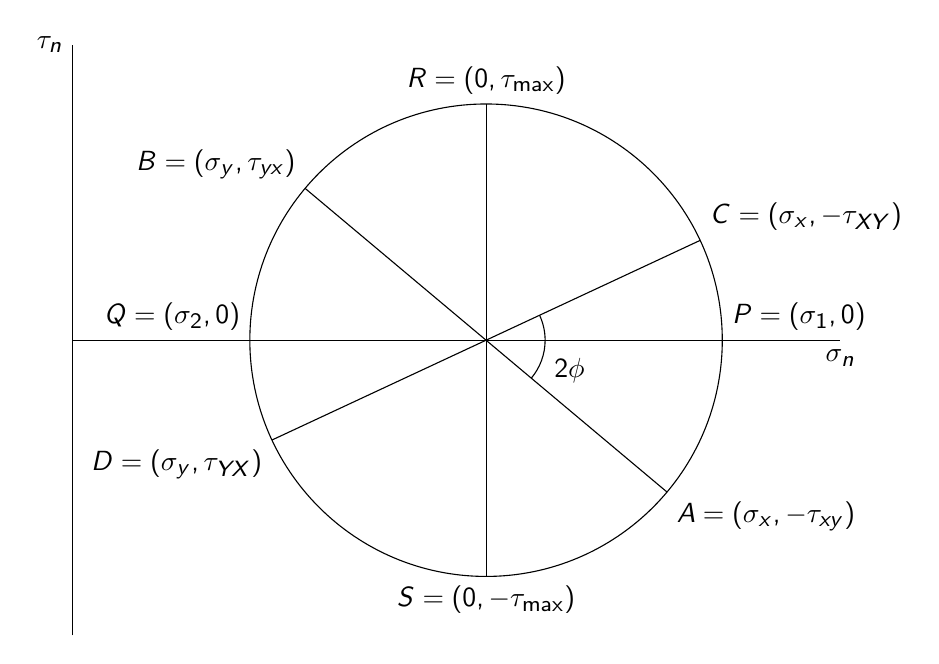
\begin{tikzpicture}[scale=0.75]

    \draw[] (-1,-5) -- (-1,5) node[pos=1.0, anchor=east] {$\tau_n$};
    \draw[] (-1,0) -- (12,0) node[pos=1.0, anchor=north] {$\sigma_n$};
    
    \draw[] (6,0) circle (4);
    
    \draw[] (2,0) -- (10,0)
    node[pos=0.0, anchor=south east] {$Q=(\sigma_2,0)$}
    node[pos=1.0, anchor=south west] {$P=(\sigma_1,0)$};
    
    \draw[] (6,-4) -- (6,4)
    node[pos=0.0, anchor=north] {$S=(0,-\tau_{\max} )$}
    node[pos=1.0, anchor=south] {$R=(0,\tau_{\max} )$};
    
    \draw[rotate around={25:(6,0)}] (2,0) -- (10,0) 
    node[pos=0.0, anchor=north east] {$D=(\sigma_y,\tau_{YX})$}
    node[pos=1.0, anchor=south west] {$C=(\sigma_x,-\tau_{XY})$};
    
    \draw[rotate around={-40:(6,0)}] (2,0) -- (10,0) 
    node[pos=0.0, anchor=south east] {$B=(\sigma_y,\tau_{yx})$}
    node[pos=1.0, anchor=north west] {$A=(\sigma_x,-\tau_{xy})$};
    
    \draw[] (7,0) arc (0:25:1);
    \draw[] (7,0) arc (0:-40:1) node[pos=0.2, anchor=north west] {$2\phi$};
    
\end{tikzpicture}
\end{document}